%! Author = anton
%! Date = 28/08/2024

Starting with the previous performance, it may be interesting to analyse how performance changes as three main
parameters vary:
\begin{itemize}
    \item \(\tilde{\pi}\): represents prior probability of the positive class
    \item \(C_{fn}\): misclassification cost of a sample predicted as negative but it is positive
    \item \(C_{fp}\): misclassification cost of a sample predicted as positive but it is negative
\end{itemize}

\begin{table}[h]
    \centering
    \begin{tabular}{>{\centering\arraybackslash}p{2.9cm} >{\centering\arraybackslash}p{2.9cm} >{\centering\arraybackslash}p{2.9cm} >{\centering\arraybackslash}p{2.9cm}}
        \toprule
        & \textbf{MVG} & \textbf{Naive Bayes} & \textbf{Tied Covariance} \\
        \midrule
        \multicolumn{4}{c}{\textbf{Application \((\tilde{\pi},C_{fn}, C_{fp}) = (0.5, 1, 1)\)}} \\
        \midrule
        \textbf{actDCF} & 0.1399       & 0.1439               & 0.1860                   \\
        \textbf{minDCF} & 0.1302       & 0.1311               & 0.1812                   \\
        \midrule
        \multicolumn{4}{c}{\textbf{Application \((\tilde{\pi},C_{fn}, C_{fp}) = (0.9, 1, 1)\)}} \\
        \midrule
        \textbf{actDCF} & 0.4001       & 0.3893               & 0.4626                   \\
        \textbf{minDCF} & 0.3423       & 0.3509               & 0.4421                   \\
        \midrule
        \multicolumn{4}{c}{\textbf{Application \((\tilde{\pi},C_{fn}, C_{fp}) = (0.1, 1, 1)\)}} \\
        \midrule
        \textbf{actDCF} & 0.3051       & 0.3022               & 0.4061                   \\
        \textbf{minDCF} & 0.2629       & 0.2569               & 0.3628                   \\
        \midrule
        \multicolumn{4}{c}{\textbf{Application \((\tilde{\pi},C_{fn}, C_{fp}) = (0.5, 1, 9)\)}} \\
        \midrule
        \textbf{actDCF} & 0.3051       & 0.3022               & 0.4061                   \\
        \textbf{minDCF} & 0.2629       & 0.2569               & 0.3628                   \\
        \midrule
        \multicolumn{4}{c}{\textbf{Application \((\tilde{\pi},C_{fn}, C_{fp}) = (0.5, 9, 1)\)}} \\
        \midrule
        \textbf{actDCF} & 0.4001       & 0.3893               & 0.4626                   \\
        \textbf{minDCF} & 0.3423       & 0.3509               & 0.4421                   \\
        \bottomrule
    \end{tabular}
    \captionsetup{justification=justified,singlelinecheck=false,format=hang}
    \caption{Table showing minDCF and actDCF for different models and applications.}
    \label{tab:resultPerformanceClassifierWithoutPCA}
\end{table}

Analysing the results of the \autoref{tab:resultPerformanceClassifierWithoutPCA}, it is possible to observe:
\begin{itemize}
    \item Observing how the \(\tilde{\pi}\) varies, it can be seen that the best outcome is obtained when it takes the value 0.5.
    On the other hand, when it takes value 0.1 and 0.9, the outcome gets worse because it penalises false negatives and false positives respectively
    \item Observing how the values of \(C_{fn}\) and \(C_{fp}\) change when they assume value 9.
    The outcomes worsen, in particular there is a greater impact on the model when the cost of false negatives increases.
\end{itemize}

Starting from the result obtained in \autoref{tab:resultPerformanceClassifierWithoutPCA}, it is possible to consider the application
of PCA as pre-processing technique focusing on the cases of \(\tilde{\pi}\) equal to 0.1, 0.5 and 0.9 and \(C_{fn}=C_{fp}=1\),
obtaining the outcomes shown in \autoref{tab:resultPerformanceClassifierWithPCA}


\begin{table}[h!]
    \centering
    \begin{tabular}{>{\centering\arraybackslash}p{2.9cm} >{\centering\arraybackslash}p{2.9cm} >{\centering\arraybackslash}p{2.9cm} >{\centering\arraybackslash}p{2.9cm}}
        \toprule
        & \textbf{MVG} & \textbf{Naive Bayes} & \textbf{Tied Covariance} \\
        \toprule
        \toprule
        \multicolumn{4}{c}{\textbf{Application \((\tilde{\pi},C_{fn}, C_{fp}) = (0.5, 1, 1)\)}} \\
        \midrule
        \multicolumn{4}{c}{\textbf{no PCA}} \\
        \midrule
        \textbf{actDCF} & 0.1399       & 0.1439               & 0.1860                   \\
        \textbf{minDCF} & 0.1302       & 0.1311               & 0.1812                   \\
        \midrule
        \multicolumn{4}{c}{\textbf{PCA}} \\
        \multicolumn{4}{c}{\textbf{\(m = 5\)}} \\
        \midrule
        \textbf{actDCF} & 0.1419       & 0.1749               & 0.1860                   \\
        \textbf{minDCF} & 0.1331       & 0.1737               & 0.1812                   \\
        \midrule
        \multicolumn{4}{c}{\textbf{\(m = 6\)}} \\
        \midrule
        \textbf{actDCF} & 0.1399       & 0.1780               & 0.1860                   \\
        \textbf{minDCF} & 0.1302       & 0.1727               & 0.1812                   \\
        \toprule
        \toprule
        \multicolumn{4}{c}{\textbf{Application \((\tilde{\pi},C_{fn}, C_{fp}) = (0.9, 1, 1)\)}} \\
        \midrule
        \multicolumn{4}{c}{\textbf{no PCA}} \\
        \midrule
        \textbf{actDCF} & 0.4001       & 0.3893               & 0.4626                   \\
        \textbf{minDCF} & 0.3423       & 0.3509               & 0.4421                   \\
        \midrule
        \multicolumn{4}{c}{\textbf{PCA}} \\
        \multicolumn{4}{c}{\textbf{\(m = 5\)}} \\
        \midrule
        \textbf{actDCF} & 0.3980       & 0.4660               & 0.4626                   \\
        \textbf{minDCF} & 0.3512       & 0.4340               & 0.4451                   \\
        \midrule
        \multicolumn{4}{c}{\textbf{\(m = 6\)}} \\
        \midrule
        \textbf{actDCF} & 0.4001       & 0.4512               & 0.4626                   \\
        \textbf{minDCF} & 0.3423       & 0.4359               & 0.4421                   \\
        \toprule
        \toprule
        \multicolumn{4}{c}{\textbf{Application \((\tilde{\pi},C_{fn}, C_{fp}) = (0.1, 1, 1)\)}} \\
        \midrule
        \multicolumn{4}{c}{\textbf{no PCA}} \\
        \midrule
        \textbf{actDCF} & 0.3051       & 0.3022               & 0.4061                   \\
        \textbf{minDCF} & 0.2629       & 0.2569               & 0.3628                   \\
        \midrule
        \multicolumn{4}{c}{\textbf{PCA}} \\
        \multicolumn{4}{c}{\textbf{\(m = 5\)}} \\
        \midrule
        \textbf{actDCF} & 0.3042       & 0.3930               & 0.4051                   \\
        \textbf{minDCF} & 0.2738       & 0.3545               & 0.3648                   \\
        \midrule
        \multicolumn{4}{c}{\textbf{\(m = 6\)}} \\
        \midrule
        \textbf{actDCF} & 0.3051       & 0.3920               & 0.4061                   \\
        \textbf{minDCF} & 0.2629       & 0.3535               & 0.3628                   \\
        \bottomrule
    \end{tabular}
    \captionsetup{justification=justified,singlelinecheck=false,format=hang}
    \caption{Show minDCF and actDCF for different models and applications before and after applying PCA.}
    \label{tab:resultPerformanceClassifierWithPCA}
\end{table}

From the results obtained in the \autoref{tab:resultPerformanceClassifierWithPCA}, it can be seen that the application of
PCA was not very helpful because in no case did the outcomes improve, instead they remained the same or even worsened.
Analysing overall, it can be said that the model that tends to perform worse is the Tied Covariance, whereas MVG and Naive
Bayes are rather similar.
In particular for MVG and Naive Bayes, the best result is obtained for the \(0.5, 1, 1\) configuration whether applying
PCA or not.
In addition, it can be said that there is a good calibration for this configuration because applying or not applying PCA,
minDCF and actDCF doesn't change what is not the case for the other configurations.

In \autoref{fig:dcfMVGNBTC} the Bayes error was calculated for a prior log odds in the range \((-4, +4)\), for the
three models with a configuration having a \(\tilde{\pi} = 0.1\) and applying the PCA as pre-processing.

\begin{figure}
    \centering
    \begin{subfigure}[b]{0.3\linewidth}
        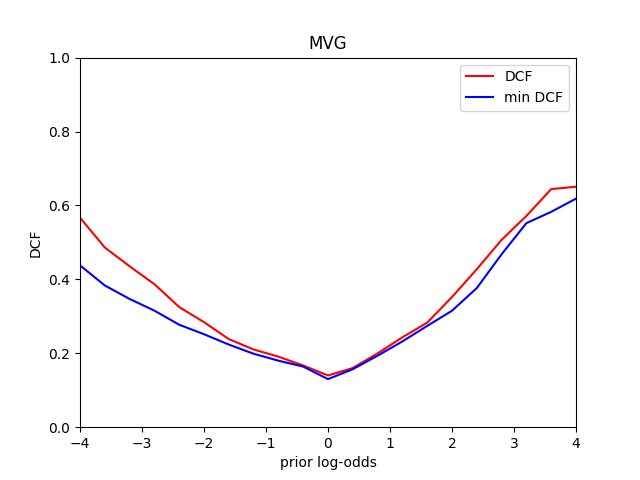
\includegraphics[width=\linewidth]{Lab/07. Lab 07/Images/01. MVG}
        \caption{MVG}
        \label{fig:dcfMVG}
    \end{subfigure}
    \begin{subfigure}[b]{0.3\linewidth}
        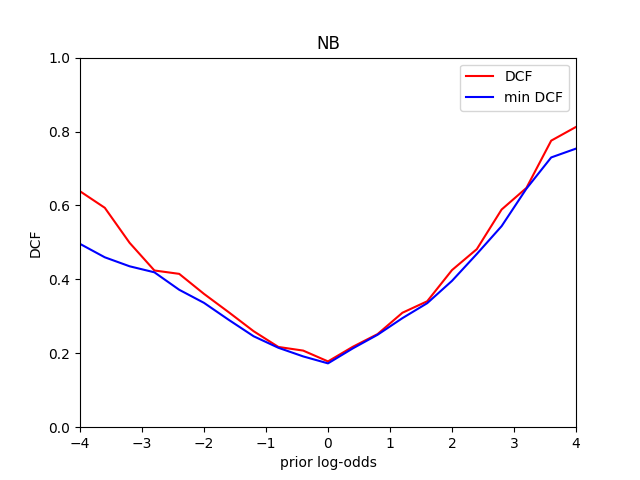
\includegraphics[width=\linewidth]{Lab/07. Lab 07/Images/02. Naive Bayes}
        \caption{Naive Bayes}
        \label{fig:dcfNB}
    \end{subfigure}
    \begin{subfigure}[b]{0.3\linewidth}
        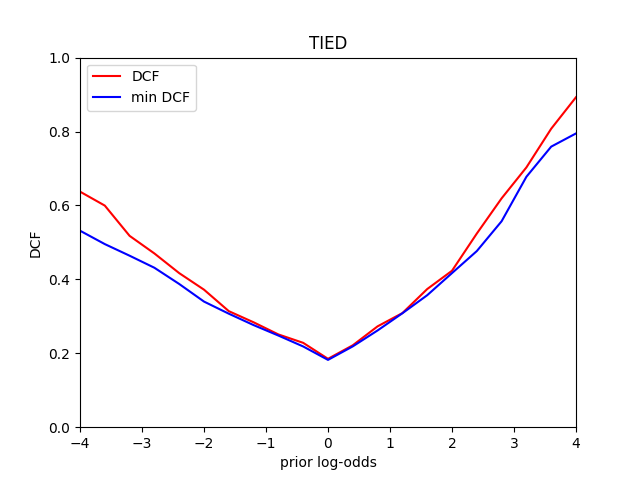
\includegraphics[width=\linewidth]{Lab/07. Lab 07/Images/03. Tied}
        \caption{Tied Covariance}
        \label{fig:dcfTC}
    \end{subfigure}
    \caption{Error Bayes plots}
    \label{fig:dcfMVGNBTC}
\end{figure}